\documentclass[12pt,a4paper,oneside]{article}
\usepackage{lscape}
\usepackage{tikz}
\usetikzlibrary{automata, positioning}
\usepackage[utf8]{inputenc}
\usepackage{graphicx}
\usepackage{algorithm}
\usepackage{algpseudocode}
\usepackage[normalem]{ulem}
\useunder{\uline}{\ul}{}
\usepackage{float}
\usepackage[none]{hyphenat}

\algnewcommand{\algorithmicand}{\textbf{ and }}
\algnewcommand{\AND}{\algorithmicand}

\date{}

\author{Gabriel Rodríguez Canal}
\title{Implementación de insertion sort mediante un diseño de máquina algorítmica}

\begin{document}

\maketitle

\section{Introducción}

En el presente documento se detalla el proceso de desarrollo de una máquina algorítmica
que implementa el algoritmo de ordenación por inserción (\textit{insertion sort}). La
implementación se ha llevado a cabo mediante el software CAD Proteus, con el procedimiento
de captura esquemática. En la sección \ref{anexo} se muestran algunas capturas del proyecto.
Se han omitido aquellas partes del mismo que, debido a sus grandes dimensiones, necesitarían 
de varias capturas para plasmarlas en el documento, por lo que perderían su propósito. Por tanto, se 
remite al lector al proyecto Proteus adjunto.\\

La máquina algorítmica se compone de la unidad de control y la unidad de proceso. La unidad 
de control implementa el autómata de control, que genera señales en función del estado de la 
máquina que son enviadas a la unidad de proceso para realizar los cálculos necesarios. La unidad 
de proceso de la máquina diseñada se detalla en la sección \ref{ud_proceso}, mientras que la unidad 
de control se describe en la sección \ref{ud_control}.

\section{Algoritmo}
A continuación se presenta el pseudocódigo del algoritmo que se ha implementado como máquina
algorítmica:

\begin{algorithm}[H]
    \caption{Insertion Sort}\label{insertion_sort}
    \begin{algorithmic}[1]
    \For {$ i = 1 $ to ${n}$}
        \State $value = arr[i]$
        \State $j = i$
        \While {$j>0 \AND arr[j-1]>value$}
            \State $arr[j] = arr[j-1]$
            \State $j = j-1$
        \EndWhile
        
        \State $arr[j] = value$
    \EndFor
    \end{algorithmic}
\end{algorithm}

Esta forma de describir el algoritmo ofrece una traducción fácil a un lenguaje de programación 
imperativo como C. Sin embargo, para la implementación como máquina algorítmica es más adecuada 
una reescritura en función de los recursos de cálculo disponibles: \\

\textbf{NOTA: A lo largo del documento se omitirá la inicialización de los registros auxiliares R1-R5 
por brevedad, sobreentendiéndose que estos estarán inicializados a 0.}\\

N=12, I=1, T=1, V=1, J=0, VALUE=0

WHILE T

{\addtolength{\leftskip}{10 mm}
VALUE=ARR[I]

J=I

WHILE V

}

{\addtolength{\leftskip}{20 mm}
ARR[J] = ARR[J-1]

J=J-1

V=CM(0, J) AND CM(VALUE, ARR[J-1])

}

ARR[J]=VALUE

I=I+1

T=CM(I, N)\\


Para una mejor comprensión del algoritmo se remite al lector a la referencia [\ref{ins_sort_ref}], en la que 
podrá, además, encontrar un vídeo explicativo del mismo.


\section{Unidad de proceso} \label{ud_proceso}
La unidad de proceso se encarga de realizar los cálculos pertinentes en función de los valores de las señales Z 
recibidos desde la unidad de control. En la subsección se detalla el flujo de la unidad de proceso, mientras que 
en la subsección \ref{esquemas} se dan los esquemas de cálculo que materializan el flujo del programa. En la 
subsección \ref{diseno} se presenta el diseño final de la unidad de proceso, resultado de los pasos anteriores.
\subsection{Planteamiento} \label{planteamiento}
\begin{table}[H]
    \begin{tabular}{lllll}
    {\ul ETAPA 1} &         &                                                                                                                &         &              \\
                  & {\ul }  & {\ul Asig. Datos}                                                                                              &         &              \\
                  &         & N=12, I=1, T=1, V=1, J=0, VALUE=0                                                                              &         &              \\
                  & {\ul }  & {\ul Salto}                                                                                                    &         &              \\
                  &         & Etapa 2                                                                                                         &         &              \\
    {\ul ETAPA 2} &         &                                                                                                                &         &              \\
                  & Si T=1: &                                                                                                                & Si T=0: &              \\
                  &         & {\ul Asig. Datos}                                                                                              &         & \textbf{FIN} \\
                  &         & \begin{tabular}[c]{@{}l@{}}VALUE=ARR{[}I{]}\\      J=I\end{tabular}                                            &         &              \\
                  &         & {\ul Salto}                                                                                                    &         &              \\
                  &         & Etapa 3                                                                                                        &         &              \\
    {\ul ETAPA 3} &         &                                                                                                                &         &              \\
                  & Si V=1: &                                                                                                                & Si V=0: &              \\
                  &         & {\ul Cálculos}                                                                                                 &         & {\ul Salto}  \\
                  &         & \begin{tabular}[c]{@{}l@{}}F1=J-1\\      F2=CM(0,F1)\\      F3=ARR{[}F1{]}\\      F4=CM(VALUE,F3)\end{tabular} &         & Etapa 4      \\
                  &         & {\ul Asig. Datos}                                                                                              &         &              \\
                  &         & \begin{tabular}[c]{@{}l@{}}ARR{[}J{]}=F3\\      J=F1\\      V=F2 AND F3\end{tabular}                           &         &              \\
                  &         & {\ul Salto}                                                                                                    &         &              \\
                  &         & Etapa 3                                                                                                        &         &              \\
    {\ul ETAPA 4} &         &                                                                                                                &         &              \\
                  &         & {\ul Cálculos}                                                                                                 &         &              \\
                  &         & \begin{tabular}[c]{@{}l@{}}F5=I+1\\      F6=CM(F5,N)\end{tabular}                                              &         &              \\
                  &         & {\ul Asig. Datos}                                                                                              &         &              \\
                  &         & \begin{tabular}[c]{@{}l@{}}ARR{[}J{]}=VALUE\\      I=F5\\      T=F6\end{tabular}                               &         &              \\
                  &         & {\ul Salto}                                                                                                    &         &              \\
                  &         & Etapa 2                                                                                                        &         &             
    \end{tabular}
    \end{table}

\subsection{Esquemas de cálculo} \label{esquemas}
\begin{figure}[H]
    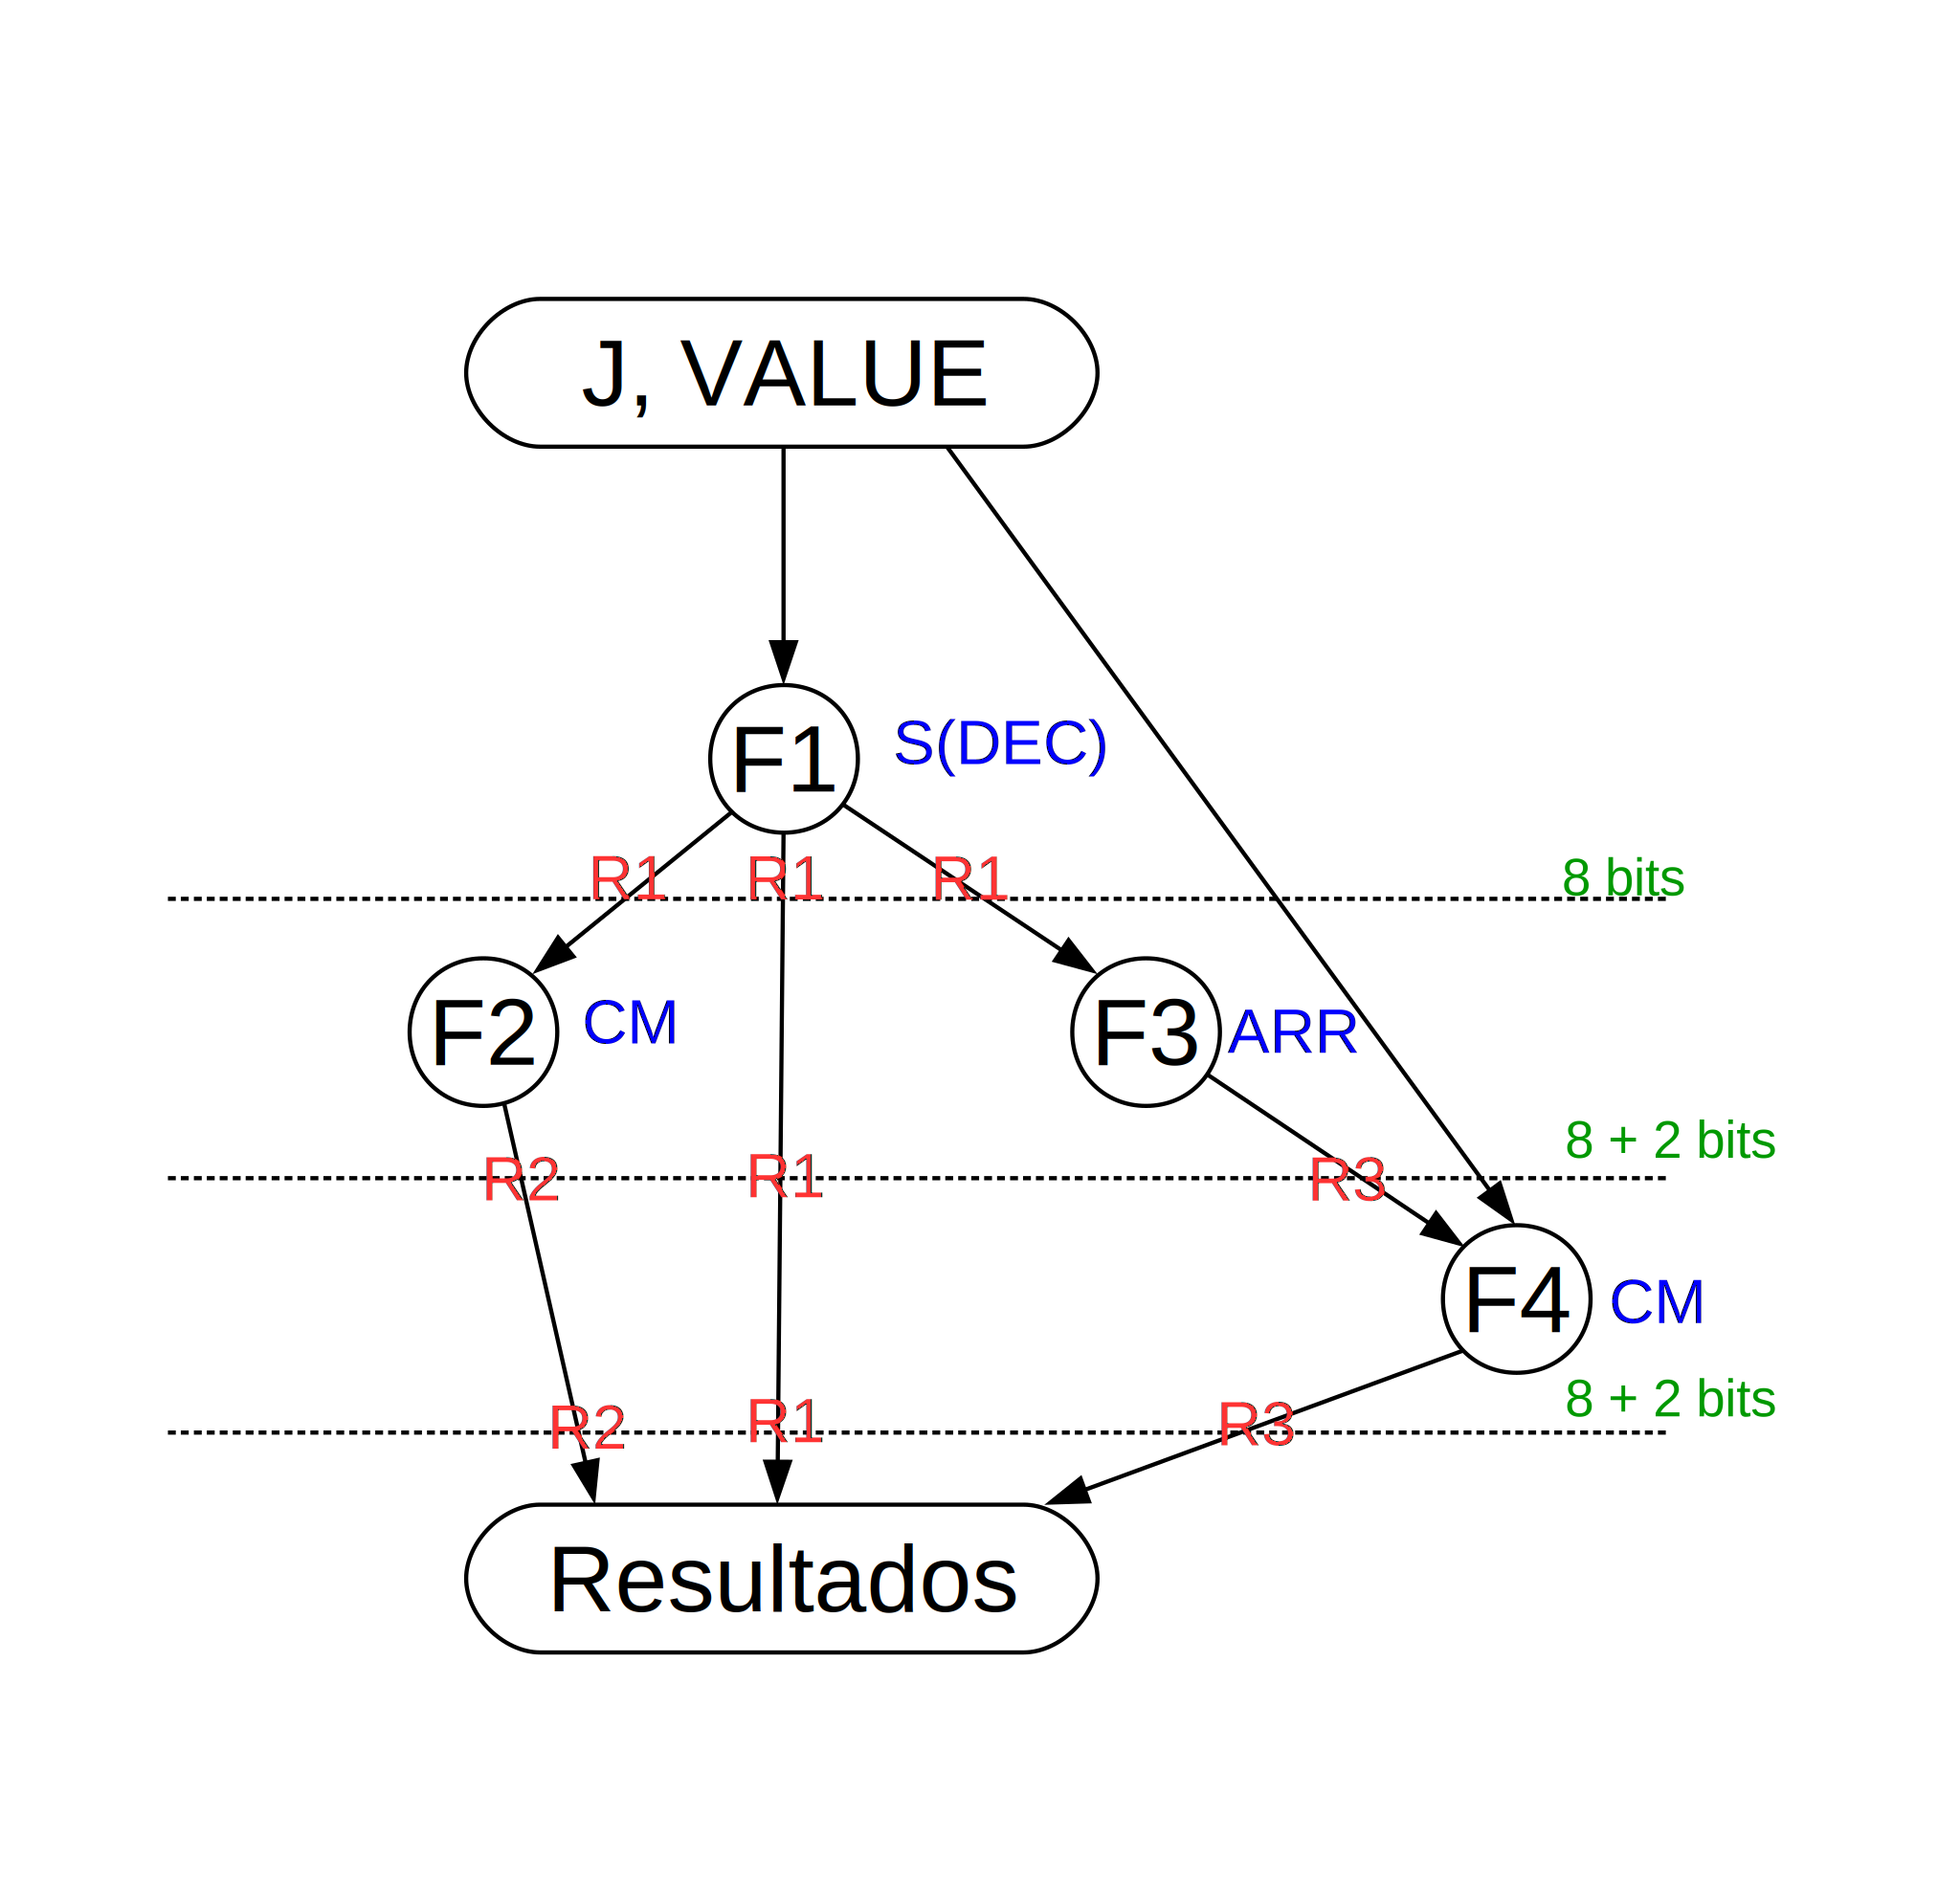
\includegraphics[width = \textwidth]{esquema1.pdf}
\end{figure}

\begin{figure}[H]
    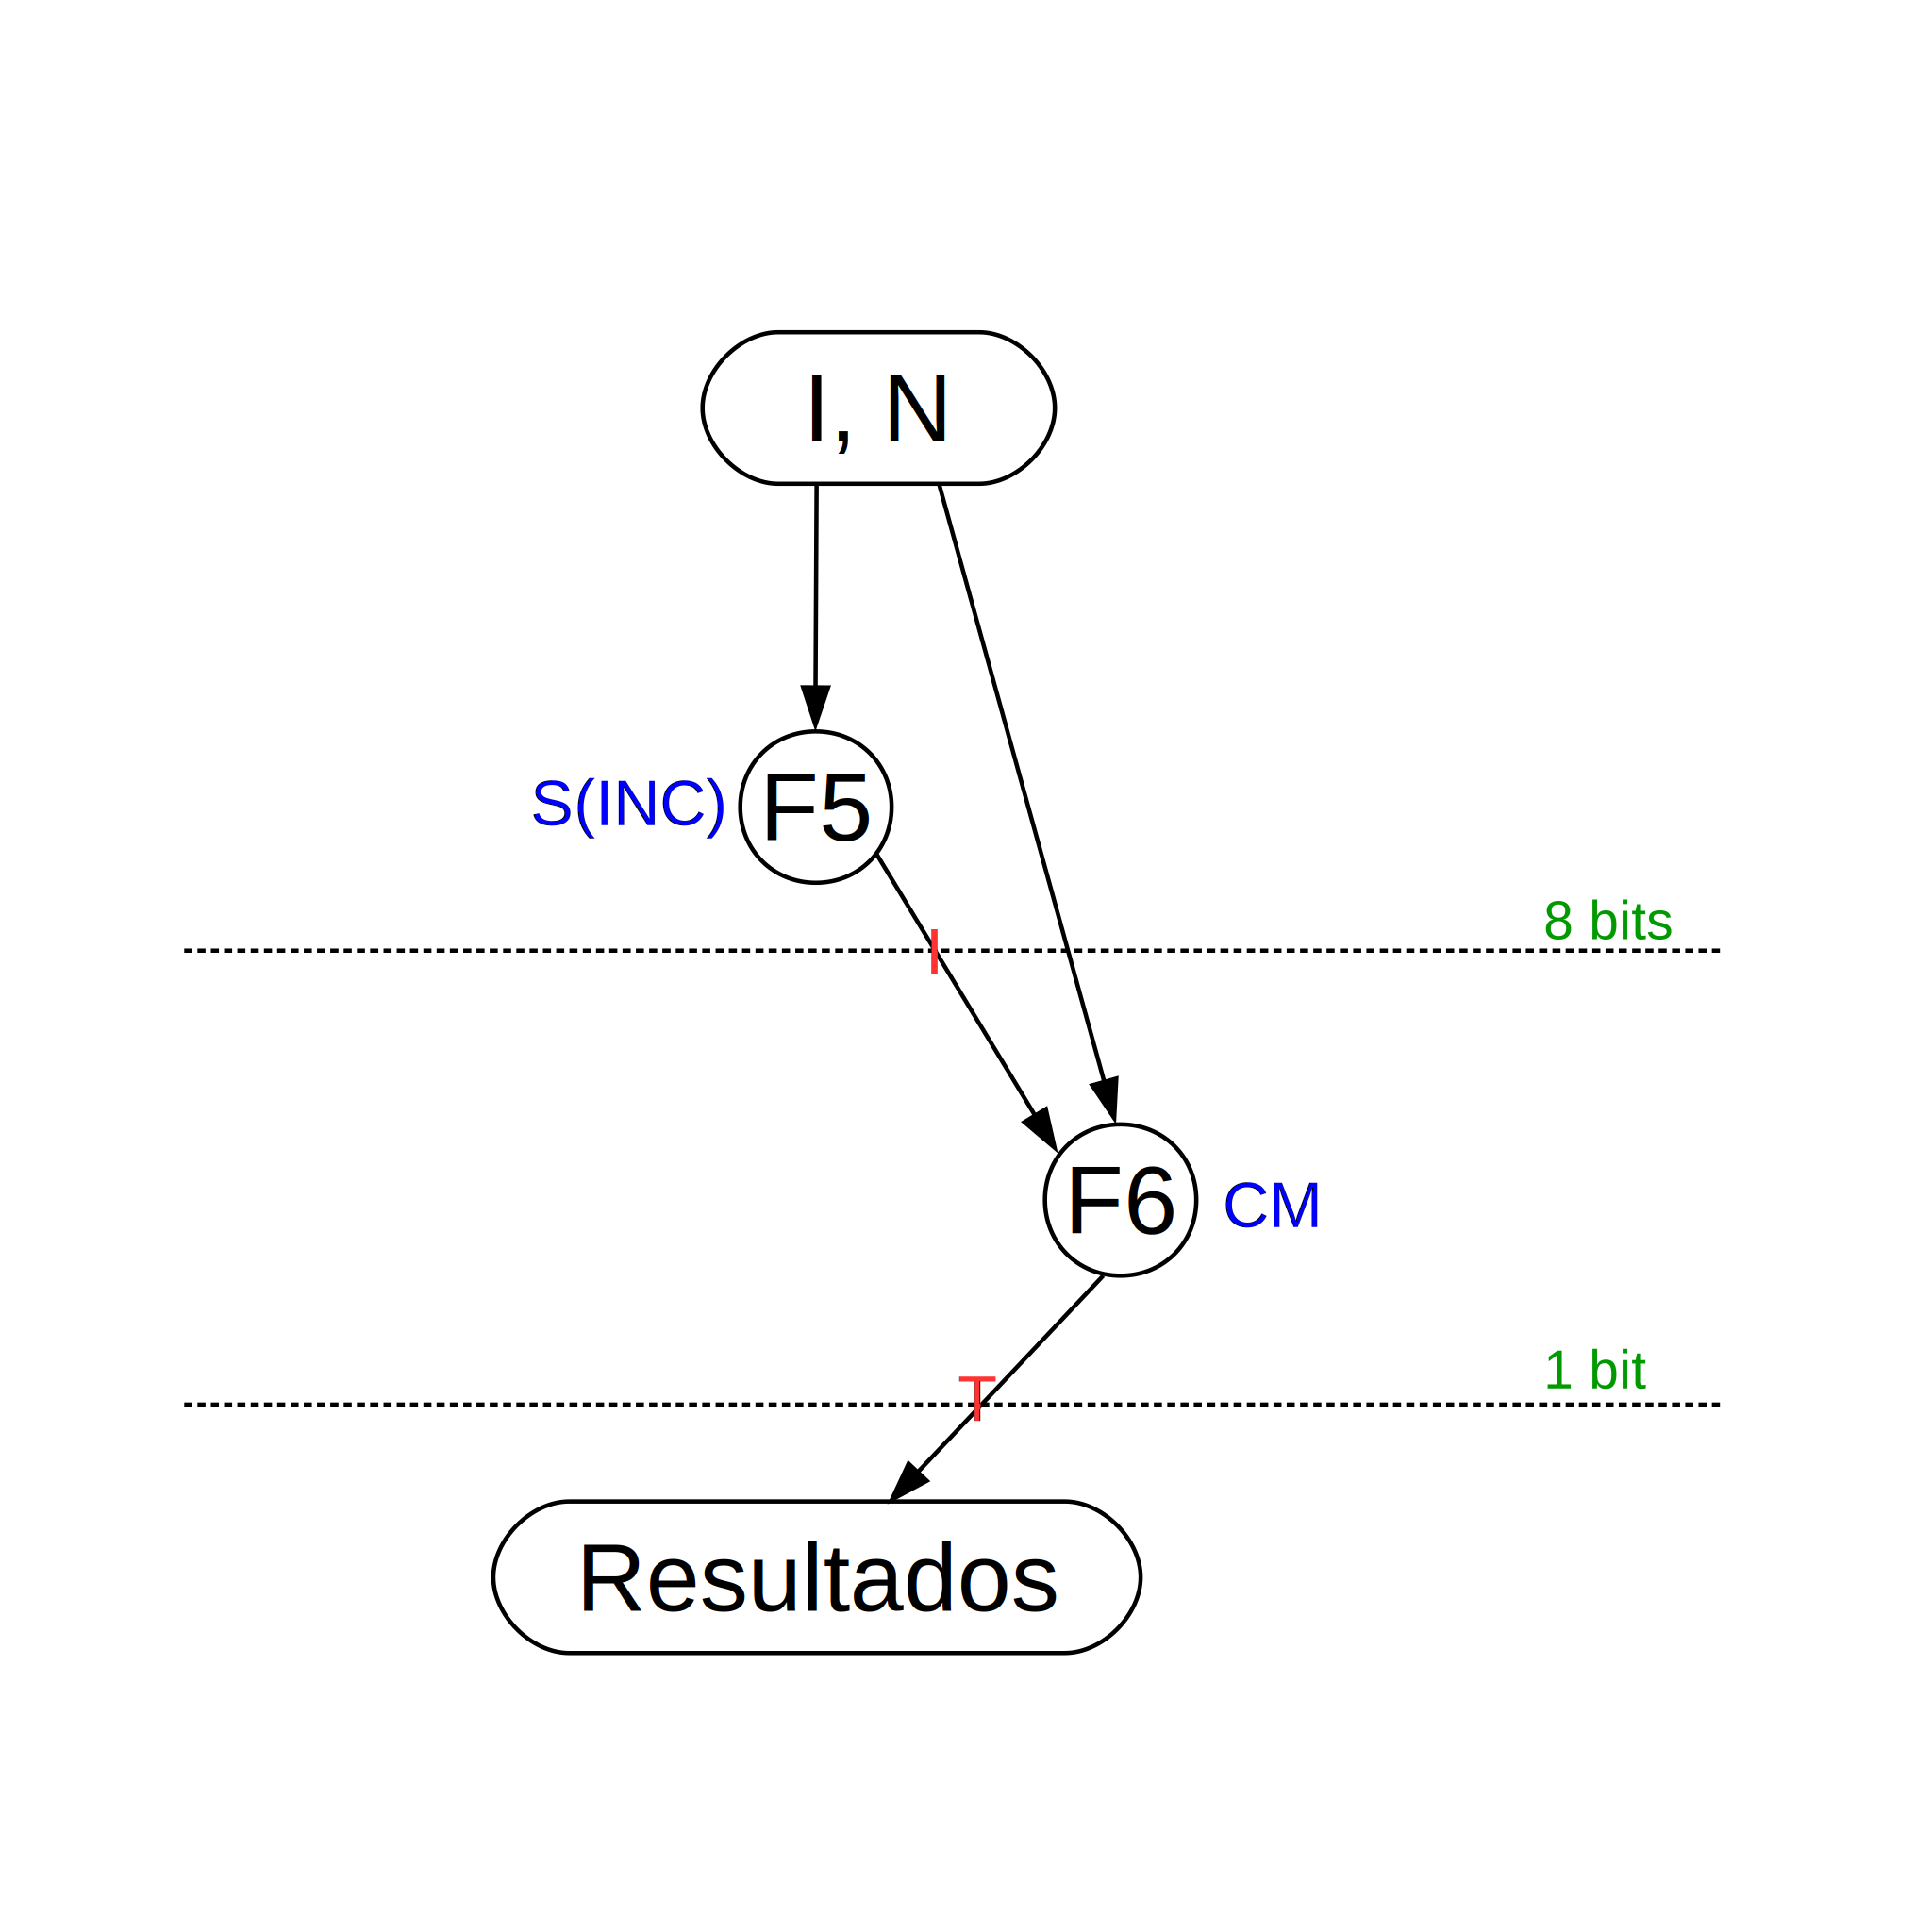
\includegraphics[width = \textwidth]{esquema2.pdf}
\end{figure}

\subsection{Asociación de recursos y registros}
\begin{figure}[H]
    \includegraphics[width = \textwidth]{asignacion-recursos.pdf}
\end{figure}

\subsection{Diseño} \label{diseno}
\begin{figure}[H]
    \includegraphics[width = \textwidth]{ud_proceso.pdf}
\end{figure}

Se ha hecho una simplificación en el circuito que calcula V. No se trata de R2 AND R3 directamente, sino
de un circuito combinacional algo más elaborado (consultar fichero Proteus para mayor detalle):

\begin{figure}[H]
    \includegraphics[width = \textwidth]{proteus-img/circuito-v-etiquetado.png}
\end{figure}

\subsection{Recurso ARR}
El recuros ARR es un array de 12 registros (N) de 8 bits. Permite la inicialización del mismo mediante su entrada 
de reloj. También existe una entrada de selección de registro. De este modo, la salida del recurso será la del registro 
seleccionado mediante esta entrada. Los valores iniciales de los registros son:

\begin{table}[] \centering
    \begin{tabular}{|c|c|c|}
    \hline
    j  & ARR{[}j{]} (DEC) & ARR{[}j{]} (HEX) \\ \hline
    0  & 23               & 17               \\ \hline
    1  & 8                & 8                \\ \hline
    2  & 1                & 1                \\ \hline
    3  & 9                & 9                \\ \hline
    4  & 6                & 6                \\ \hline
    5  & 45               & 2D               \\ \hline
    6  & 7                & 7                \\ \hline
    7  & 6                & 6                \\ \hline
    8  & 10               & A                \\ \hline
    9  & 30               & 1E               \\ \hline
    10 & 62               & 3E               \\ \hline
    11 & 24               & 18               \\ \hline
    \end{tabular}
    \caption{Valores iniciales de los registros del recurso ARR} \label{val_inic}
\end{table}



\section{Unidad de control} \label{ud_control}
La unidad de control se encarga de generar las señales Z que indican a la unidad de proceso qué 
cálculo ha de efectuar en la etapa actual. Implementa el autómata de control (subsección \ref{aut_control}), que depende del estado 
de la máquina (codificado mediante $y_2$, $y_1$ e $y_0$), de la señal de INICIO y de los bits T y V, 
que proceden de la unidad de proceso. Pese a que se presente el esquema de la unidad de control como 
un PLD programable, en realidad se ha implementado en Proteus mediante puertas NAND (ver anexo y proyecto adjunto).
El programa de control (subsección \ref{prog_control}) y el autómata de control son dos 
representaciones equivalentes del flujo seguido por la máquina de estados. En la subsección \ref{senales} se 
detallan todas las señales generadas por la unidad de control.
\begin{figure}[H]
    \includegraphics[width = \textwidth]{ud_control.pdf}
    \caption{Esquema de la unidad de control}
\end{figure}

\subsection{Programa de control} \label{prog_control}
\begin{table}[H]
    \begin{tabular}{llll}
    1: &                    & , {[}N=12, I=1, T=1, V=1, J=0, VALUE=0{]} & , 2; \\
    2: & T                  & , {[}VALUE=ARR{[}I{]}, J=I{]}             & , 3; \\
       & \=T & , FIN                                     &      \\
    3: &                    & , {[}R1=S(J,-1), R5=J{]}                  & , 4; \\
    4: &                    & , {[}R2=CM(0,J), R3=ARR{[}R1{]}{]}        & , 5; \\
    5: &                    & , R3=CM(VALUE,R3)                         & , 6; \\
    6: &                    & , {[}V=R2 AND R3, R4=ARR{[}R1{]}{]}       & , 7; \\
    7: & V                  & , {[}ARR{[}R5{]}=R4, J=R1{]}              & , 3; \\
       & \=V & , {[}I=S(I,1), ARR{[}J{]}=VALUE{]}        & , 8; \\
    8: &                    & , T=CM(I,N)                               & , 2;
    \end{tabular}
\end{table}

\subsection{Diagrama de flujo (Autómata de control)} \label{aut_control}
\begin{figure}[H]
\begin{tikzpicture}[shorten >=1pt,node distance=2.5cm,on grid,auto] 
    \node[state,initial] (A)   {$1$}; 
    \node[state] (B) [below of=A] {$2$}; 
    \node[state] (C) [below of= B] {$3$}; 
    \node[state] (D) [below of= C] {$4$};
    \node[state] (E) [below of=D] {$5$};
    \node[state] (F) [below of=E] {$6$};
    \node[state] (G) [below of=F] {$7$};
    \node[state] (H) [right =7cm of G] {$8$};
     \path[->] 
     (A) edge  node {INICIO=1/PRESET} (B)
     (B) edge  node  {T=1/SETVALYJ} (C)
     (C) edge  node {*/DEC} (D) 
     (D) edge node {*/COMPYGETARR} (E)
     (E) edge node {*/COMPYSETJ} (F)
     (F) edge node {*/SETV} (G)
     (G) edge node [swap]{V=0/INCYSETARR} (H);
     \draw[->] (H) |- node[below right, pos = 0.1]{*/HASENDED} (B);
     \draw[->] (G)  -| node[below, pos = 0.25]{V=1/SETARRJ} (-6,-5)  --  (C);
 \end{tikzpicture}
 \caption{Autómata de control}
\end{figure}


\subsection{Señales} \label{senales}

\begin{table}[H]
    \begin{tabular}{|l|l|cc|}
    \hline
    Orden       & Operaciones                             & \multicolumn{1}{l}{Z1} & \multicolumn{1}{l|}{Z2}  \\ \hline
    PRESET      & N=12, I=1, V=1, J=0, VALUE=0, INIC(ARR) & *                       & *                      \\ \cline{1-2} \hline
    INCYSETARR  & I=S(I,1), ARR{[}J{]}=VALUE              & 0                       & *                      \\ \cline{1-2} \hline
    DEC         & R1=S(J-1), R5=J                         & 1                       & *                      \\ \cline{1-2} \hline
    COMPYGETARR & R2=CM(0,J), R3=ARR{[}R1{]}              & *                       & 0                      \\ \cline{1-2} \hline
    COMPYSETJ   & R3=CM(VALUE,R3)                         & *                       & 1                      \\ \cline{1-2} \hline
    SETV        & V=R2 AND R3, R4=ARR{[}R1{]}             & *                       & *                      \\ \cline{1-2} \hline
    HASENDED    & T=CM(I,N)                               & *                       & 2                      \\ \cline{1-2} \hline
    SETVALYJ    & VALUE=ARR{[}I{]}, J=I, V=1              & *                       & *                      \\ \cline{1-2} \hline
    NOOP        & No hace nada                            & *                       & *                      \\ \cline{1-2} \hline
    SETARRJ     & ARR{[}R5{]}=R4, J=R1                    & *                       & *                      \\ \cline{1-2} \hline
    \end{tabular}
\end{table}
\begin{table}[H]
    \begin{tabular}{|l|ccccccccccc|}
    \hline
    Orden           & \multicolumn{1}{l}{Z3}  & \multicolumn{1}{l}{Z4}  & \multicolumn{1}{l}{Z5}  & \multicolumn{1}{l}{Z6}  & \multicolumn{1}{l}{Z7}  & \multicolumn{1}{l}{Z8}  & \multicolumn{1}{l}{Z9}  & \multicolumn{1}{l}{Z10} & \multicolumn{1}{l}{Z11} & \multicolumn{1}{l}{Z12} & \multicolumn{1}{l|}{Z13} \\ \hline
    PRESET          & *                       & *                       & 1                       & 0                       & 0                       & 0                       & 0                       & 0                        & 0                       & 0                       & 0                       \\ \cline{1-2} \hline
    INCYSETARR      & 1                       & *                       & 0                       & 0                       & 0                       & 0                       & 0                       & 1                        & 0                       & 0                       & 1                       \\ \cline{1-2} \hline
    DEC             & *                       & *                       & 0                       & 1                       & 0                       & 0                       & 0                       & 0                        & 0                       & 0                       & 0                       \\ \cline{1-2} \hline
    COMPYGETARR     & 0                       & 1                       & 0                       & 0                       & 1                       & 1                       & 0                       & 0                        & 0                       & 0                       & 0                       \\ \cline{1-2} \hline
    COMPYSETJ       & 0                       & 0                       & 0                       & 0                       & 0                       & 1                       & 0                       & 0                        & 0                       & 0                       & 0                       \\ \cline{1-2} \hline
    SETV            & 0                       & *                       & 0                       & 0                       & 0                       & 0                       & 0                       & 0                        & 0                       & 0                       & 0                       \\ \cline{1-2} \hline
    HASENDED        & *                       & *                       & 0                       & 0                       & 0                       & 0                       & 0                       & 0                        & 0                       & 1                       & 0                       \\ \cline{1-2} \hline
    SETVALYJ        & *                       & *                       & 0                       & 0                       & 0                       & 0                       & 1                       & 0                        & 1                       & 0                       & 0                       \\ \cline{1-2} \hline
    NOOP            & *                       & *                       & 0                       & 0                       & 0                       & 0                       & 0                       & 0                        & 0                       & 0                       & 0                       \\ \cline{1-2} \hline
    SETARRJ         & 0                       & *                       & 0                       & 0                       & 0                       & 0                       & 0                       & 0                        & 1                       & 0                       & 1                       \\ \cline{1-2} \hline
    \end{tabular}
\end{table}
\begin{table}[H]
    \begin{tabular}{|l|cccc|}
    \hline
    Orden              & \multicolumn{1}{l}{Z14} & \multicolumn{1}{l}{Z15} & \multicolumn{1}{l}{Z16} & \multicolumn{1}{l|}{Z17} \\ \hline
    PRESET             & *                       & *                       & 0                       & 0                        \\ \cline{1-2} \hline
    INCYSETARR         & 1                       & *                       & 0                       & 0                        \\ \cline{1-2} \hline
    DEC                & *                       & *                       & 0                       & 0                        \\ \cline{1-2} \hline
    COMPYGETARR        & 0                       & *                       & 0                       & 0                        \\ \cline{1-2} \hline
    COMPYSETJ          & 0                       & 0                       & 0                       & 1                        \\ \cline{1-2} \hline
    SETV               & 0                       & *                       & 1                       & 1                        \\ \cline{1-2} \hline
    HASENDED           & *                       & *                       & 0                       & 0                        \\ \cline{1-2} \hline
    SETVALYJ           & 2                       & 1                       & 0                       & 0                        \\ \cline{1-2} \hline
    NOOP               & *                       & *                       & 0                       & 0                        \\ \cline{1-2} \hline
    SETARRJ            & 3                       & 0                       & 1                       & 0                        \\ \cline{1-2} \hline
    \end{tabular}   
    \caption{Señales de la unidad de control.}
\end{table}

\section{Comprobación de funcionamiento del circuito}
Para comprobar el funcionamiento del circuito se sugiere al lector hacer una simulación con el gráfico digital de la 
unidad de proceso. Entre otros, se monitorizan las sondas ARR0[0..7], ARR1[0..7], ..., ARR11[0..7], que comienzan la 
ejecución con los valores de la tabla \ref{val_inic} y terminar ordenados.

\section{Anexo} \label{anexo}
\begin{figure}[H]
    \includegraphics[width = \textwidth]{proteus-img/raiz.PNG}
    \caption{Hoja raíz}
\end{figure}

\begin{figure}[H]
    \includegraphics[width = \textwidth]{proteus-img/ud_control.PNG}
    \caption{Unidad de control}
\end{figure}

\begin{figure}[H]
    \includegraphics[width = \textwidth]{proteus-img/controlandor.PNG}
    \caption{Detalle del bloque CONTROLANDOR}
\end{figure}

\begin{figure}[H]
    \includegraphics[width = \textwidth]{proteus-img/ycontrol.PNG}
    \caption{Detalle del bloque YCONTROL}
\end{figure}

\begin{figure}[H]
    \includegraphics[width = \textwidth]{proteus-img/selectbitscontrol.PNG}
    \caption{Detalle del bloque SELECTBITS}
\end{figure}

\begin{figure}[H]
    \includegraphics[width = \textwidth]{proteus-img/muxzcontrol.PNG}
    \caption{Detalle del bloque MUXZ}
\end{figure}

\begin{figure}[H]
    \includegraphics[width = \textwidth]{proteus-img/registro.PNG}
    \caption{Detalle del bloque REGISTRO}
\end{figure}

\begin{figure}[H]
    \includegraphics[width = \textwidth]{proteus-img/arr.PNG}
    \caption{Detalle del recurso ARR}
\end{figure}

\begin{figure}[H]
    \includegraphics[width = \textwidth]{proteus-img/arr-selec-0.PNG}
    \caption{Detalle del combinacional de selección del registro 0 del bloque ARR}
\end{figure}

\section{Referencias}
\begin{enumerate}
\item Marqués Cuesta, Luis Alberto. "Diseño de Hardware Específico - Tema 5: Esquemas de cálculo". Universidad de Valladolid.
\item Marqués Cuesta, Luis Alberto. "Diseño de Hardware Específico - Tema 6: Máquinas algorítmicas". Universidad de Valladolid.
\item P. Deschamps y J.M. Angulo, Diseño de sistemas digitales, metodología moderna, Paraninfo. 
\item Fecha de consulta: 05/05/2019. Insertion sort. Obtenido de \\
https://www.geeksforgeeks.org/insertion-sort/ \label{ins_sort_ref}
\end{enumerate}

\end{document}

